%----------------------------------------------------------------------------------------
%	PACKAGES AND THEMES
%----------------------------------------------------------------------------------------
\documentclass[aspectratio=169,xcolor=dvipsnames]{beamer}
\usetheme{SimplePlus}

\usepackage{hyperref}
\usepackage{graphicx} % Allows including images
\usepackage{booktabs} % Allows the use of \toprule, \midrule and \bottomrule in tables
\usepackage{pdfpages}

\usepackage{lineno}
\usepackage{graphicx} 
\usepackage{subcaption}
\usepackage{amsmath}
\usepackage{booktabs}
\usepackage{float}


%----------------------------------------------------------------------------------------
%	TITLE PAGE
%----------------------------------------------------------------------------------------

\title{The Role of Media Coverage in Shaping Household Inflation Expectations: An Analysis of ECB Press Conferences and News Reporting} 

\author[authors] {Jasper Bär}

%----------------------------------------------------------------------------------------
%	PRESENTATION SLIDES
%----------------------------------------------------------------------------------------

\begin{document}

\begin{frame}[noframenumbering,plain]
    % Print the title page as the first slide
    \titlepage
\end{frame}

%------------------------------------------------
\section{First Section}
%------------------------------------------------

\begin{frame}{Main Idea}

\begin{itemize}
	\item How does media coverage influences inflation expectations?
	\item 
\end{itemize}

\end{frame}

%------------------------------------------------

\begin{frame}{Model}

\begin{itemize}
	\item I follow Lamla and Lein (2014) and use a Bayesian Learning framework for forming my hypothesis.
	\item The central bank sends a normally distributed signal $c_t$ about the central bank inflation forecast to the media.
	\item Without the central bank the media would send a normally distributed "baseline" signal about the future inflation $s_{\nu,t}^b$ for a number of media report $V$. 
	\item The media sends a signal $s_{\nu,t}$ about the future inflation which is the weighted average of the central banks signal and the "baseline" signal. 
	\begin{align*}
s_{\nu,t} = (1-\lambda_{\nu,t}) s^b_{\nu,t} + \lambda_{\nu,t} c_t \quad 0\leq \lambda_{\nu,t} \leq 1 \\
\end{align*}
\end{itemize}

\end{frame}

%------------------------------------------------

\begin{frame}{Model}

\begin{itemize}
	\item Given that $s_{\nu,t}$ is a linear combination of normal random variables and assuming that $\sigma^c_t$ and $\sigma^{sb}{\nu,t}$ are independent, the media sends a normally distributed signal about $\pi{t+1}$ with $s_{\nu,t} \sim N(\mu^s_{\nu,t}, \sigma^s_{\nu,t})$, where:
\begin{equation} 
\mu_{\nu,t}^s = (1-\lambda_{\nu,t}) (\alpha_t + \Psi_t) + \lambda_{\nu,t} \Theta_t 
\end{equation}
	\item The households hold a prior belief $\gamma_t \sim N(\pi_t, \sigma^h_t)$ about the future inflation.
	\begin{align*}
s_{\nu,t} = (1-\lambda_{\nu,t}) s^b_{\nu,t} + \lambda_{\nu,t} c_t \quad 0\leq \lambda_{\nu,t} \leq 1 \\
\end{align*}
\end{itemize}

\end{frame}

%------------------------------------------------

\begin{frame}{Data}

\begin{itemize}
	\item Newspaper Dataset from Dpa. I could also add "Die Welt" once the datset is ready.
	\item All sentences which contain the word "Inflation" or its synonyms like "Preissteigerung" (price increase) are identified as inflation related.
	\item ECB press conferences are downloaded from the official ECB website and cleaned.
\end{itemize}

\end{frame}

%------------------------------------------------

\begin{frame}{Measuring Media Bias}

\begin{itemize}
	\item I annotated 3000 sentences from the Newspaper articles and the ECB press conferences.
	\item I used a method from Shapiro et al. (2022) based on PMI to create lexicons for the two datasets.
	\item Newspaper articles sentences are classified into "Inflation Direction" and "Inflation Sentiment".
	\item ECB press conferences are classified into "Inflation Direction".
	\item Dependency parsing is used to identify all sentences in which the ECB is directly or indirectly cited.
\end{itemize}

\end{frame}

%------------------------------------------------

\begin{frame}{Measuring Media Bias}

 \begin{figure}[!ht]
    \centering
    \setkeys{Gin}{width=\linewidth,height=6cm} %set image parameters
    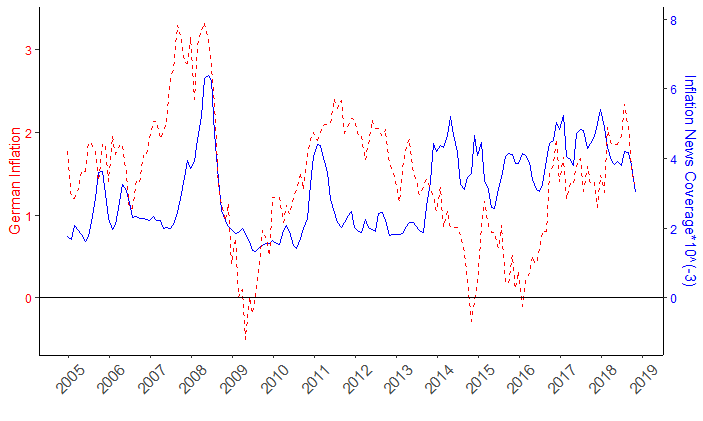
\includegraphics{Inflation_Count.png}
    \end{figure}

\end{frame}

%------------------------------------------------

\begin{frame}{Measuring Media Bias}

 \begin{figure}[!ht]
    \centering
    \setkeys{Gin}{width=\linewidth,height=6cm} %set image parameters
    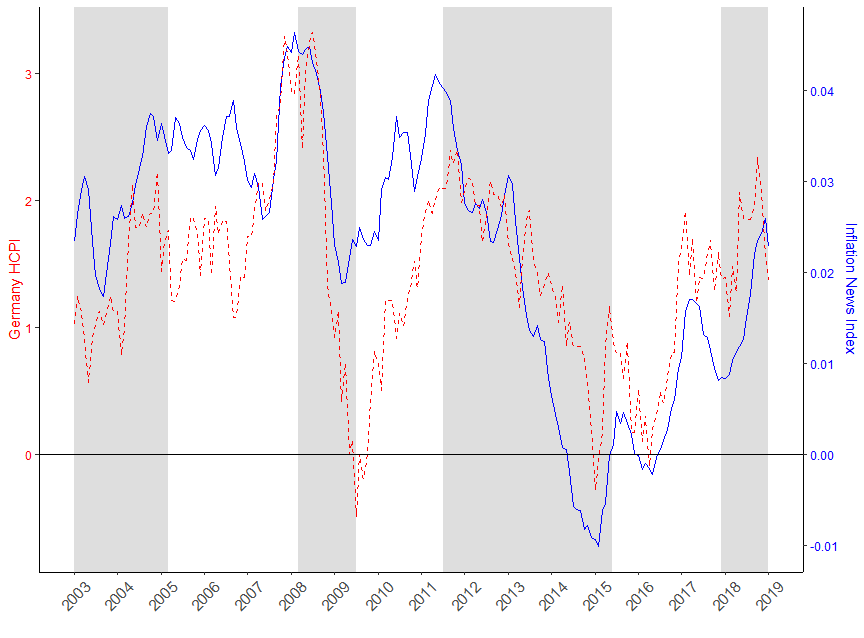
\includegraphics{Inflation_Sentiment_Direction.png}
    \label{Inflation_Sentiment_Direction}
    \end{figure}

\end{frame}

%------------------------------------------------


\begin{frame}{Measuring Media Bias}

Plots

\end{frame}

%------------------------------------------------

\begin{frame}{Inflation Expectations Gap}

\begin{itemize}
\item I follow Lamla and Lein (2014) and measure the inflation expectations gap as the quantified inflation forecast and the professional one-year-ahead forecasts.
\item Several quantification methods exist. 
\item Quantification methods are barely mentioned after 2014. Why?
\end{itemize}

\end{frame}

%------------------------------------------------

\begin{frame}{Inflation Expectations Gap}

Plot

\end{frame}

%------------------------------------------------

\end{document}